%\externaldocument{ifcg/evaluation}

We conduct our parallel experiments on a 16-cores node composed of two 8-core Intel Xeon\textsuperscript{\textregistered} processors E5-2670 at 2.6 GHz and a 20 MB L3 shared cache memory with SuSe Linux OS. 
%In order to instrument and visualize the execution details we use the Paraver \cite{paraver} and Extrae \cite{extrae} tool sets. 
All the algorithms we consider in the evaluation (IFCG1, IFCG2, Preconditioned CG, Pipelined CG~\cite{ghysels14}, Chronopoulos CG~\cite{chronopoulos89} and 
Gropp CG~\cite{gropp10}) are implemented using the OpenMP4.0 programming model running on top of the Nanos++ (v0.7a) parallel runtime system~\cite{nanos}. 
We use the Intel's MKL~\cite{mkl} library to compute the fundamental linear algebra kernels involved in our experiments. 
All the aforementioned algorithms are implemented with the Block-Jacobi preconditioner with incomplete Cholesky factorization within the blocks. The block size N is 
set to 64 throughout the experiments and the convergence threshold is $||b-Ax_{i}||_{2}/||b||_{2} < 10^{-7}$

We consider 7 Symmetric and Positive Definite (SPD) matrices from The University of Florida Sparse Matrix Collection~\cite{florida}.
We use two matrices from circuit simulation problems (\emph{G3\_circuit} and \emph{G2\_circuit}), two matrices from unstructured Finite Element Method schemes (\emph{thermal2}, \emph{consph}), one matrix from material engineering problems (\emph{af\_shell8}) and one matrix from a computational fluid dynamics problem (\emph{cfd2}). % and a 3D mesh problem matrix (\emph{nd24K}). 
In Table~\ref{table:ifcg_matrices} we show a more precise description of all considered matrices in terms of their dimensions and sparsity.
The considered matrices cover a wide range of dimensions (from 72,000 up to 1,585,478 rows and columns) and sparsity degrees, which makes them representative of the typical problems faced by the CG method and its variants.

%When running all considered CG variants, the convergence threshold is setup to $10^{-7}$.

\begin{figure*}[bhtp]
        %\centerline{\includegraphics[width=\textwidth, trim={0cm 0 0cm 0},clip]{figs/aaa.pdf}}
        \centerline{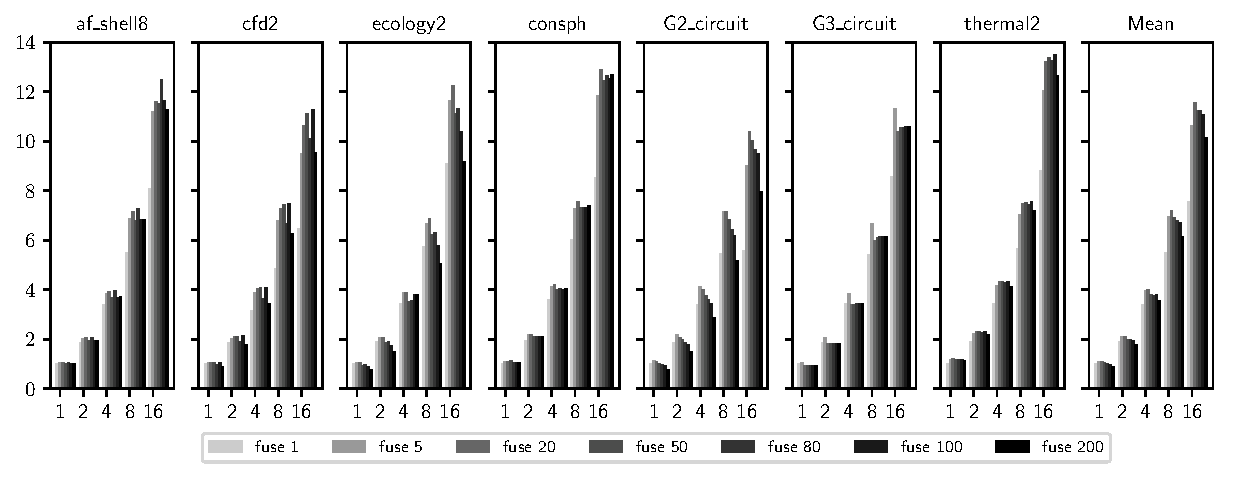
\includegraphics[width=\textwidth, trim={0cm 0 0cm 0},clip]{ifcg/figs/mn3_fuse/cg_speedup_bar_nd.pdf}}
		%\centerline{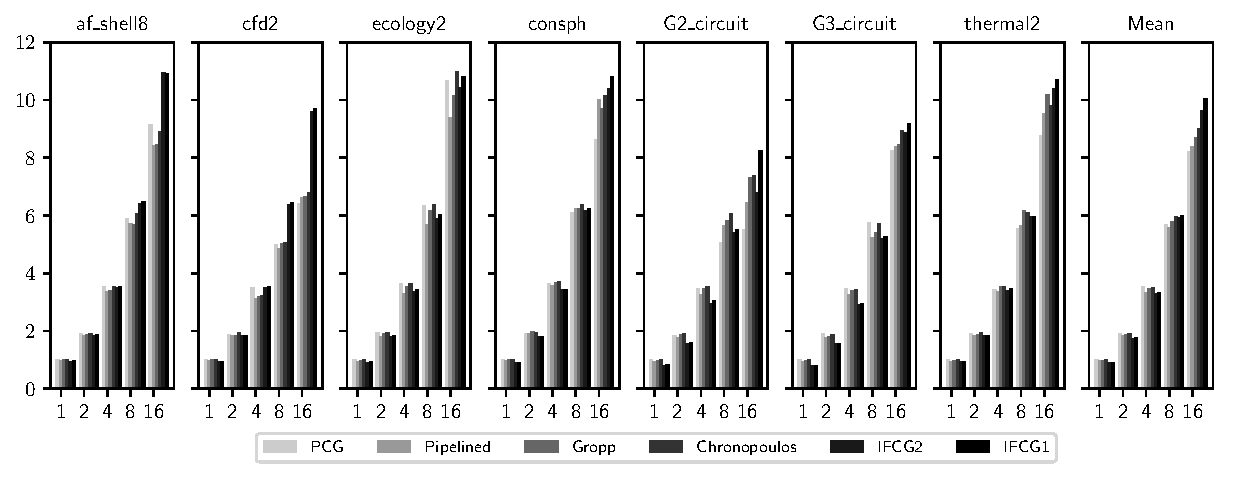
\includegraphics[width=\textwidth, trim={2.5cm 0 2.5cm 0},clip]{figs/mn3_comp/cg_speedup_bar2.pdf}}
        %\vspace{-0.75cm}
        \caption{Impact of the \emph{FUSE} parameter on IFCG1. The y-axis represents the achieved speedups with respect to the \emph{FUSE}=1 configuration running on 1 core while x-axis represents core counts.}
        \label{fuse}
\end{figure*}
